\chapter{Analytical Needle Probe Approach}
\label{sec:analytical-np}
\bigskip

\section{Introduction}
\label{sec:analytical-np:intro}

The technique used to measure thermal conductivity with a needle probe is based
on the assumption that the needle approximates an infinite line source of energy
with a constant heat flux embedded in an infinite medium. The origins of the
analytical solution for isotropic thermal conductivity may be found in Carslaw
and Jaeger's book, ``Conduction of Heat in Solids.''
\marginpar{Need to bibtex up my sources!}

The method based on Carslaw and Jaeger's solution depends on solving a 2-D
problem, where all planes orthogonal to the needle have the same temperature
distribution; in other words, temperature is not a function of axial position.
Moreover, the problem is further simplified by posing the problem into radial
coordinates and solving for temperature as a function of radial distance only.

In the isotropic case, this is straightforward, as conductivity is a constant
scalar. Unfortunately, the anisotropic case is more complex, but luckily not
completely intractible.

\section{The Isotropic Case}
\label{sec:analytical-np:isotropic}

The isotropic case solves the following equation:

\begin{equation*}
-k\nabla^2 T = \rho C\frac{\partial T}{\partial t}
\end{equation*}

Where \(T\) is temperature, \(k\) is a scalar thermal conductivity, \(\rho\) is
density, \(C\) is volumetric heat capacity, and \(t\) is time.

\marginpar{From Carslaw \& Jaeger, pg. 261}

By casting this problem into cylindrical coordinates, the equations may be
simplified such that they are a function of radial distance \(r\) only (as
temperature is assumed to not be a function of axial position \(z\) or angle
\(\phi\)).

After applying this transformation and solving the equation, the analytical
solution to the problem becomes:

\begin{equation}
\label{isotropic_ei}
T(r,t) = - \frac{q}{4\pi k}\Ei\left(-\frac{r^2}{4kt}\right)
\end{equation}

where \(q\) is heat flux from the needle per linear distance.

Solving for the exponential integral analytically is not possible, and numerical
solutions can be difficult. Typically, we instead use an approximation for small
\(r/t\),

\begin{equation}
\label{isotropic_case}
T(r,t) = \frac{q}{4\pi K}\ln\left(\frac{4Kt}{r^2}\right) - \frac{\gamma q}{4\pi K}
\end{equation}

Typical use of this function is to find \(\frac{dT}{d(\ln t)}\) and solve that
for \(k\). We will be working with \ref{isotropic_case} for the remainder of
this analysis, though it could easily be applied to \ref{isotropic_ei} as well.


\section{Difficulties In The Anisotropic Case}
\label{sec:analytical-np:anisotropic-diff}


The anisotropic case varies from the isotropic one in that instead of a scalar 
thermal conductivity \(k\), one must solve the problem using an \(n \times n\)
thermal conductivity, \([K]\), where \(n\) is the number of dimensions in the
problem. As a consequence, reducing the problem into two dimensions becomes more
difficult. Moreover, when the problem is posed in cylindrical coordinates, the
solution becomes a function not only of \(r\), but of \(\phi\) as well.

\section{Posing The Problem in Two Coordinates}
\label{sec:analytical-np:2D}

By assuming that temperature distribution is not a function of axial direction
\(z\), we may reduce the problem to an analogous one in orthogonal directions
\(x\) and \(y\) instead:

\begin{equation}
-\nabla_{xy} \cdot \left([K]_{2 \times 2}\nabla_{xy} T \right)= \rho C\frac{\partial T}{\partial t}
\end{equation}

Without loss of generality, it may be further simplified like so:

\begin{equation}
-\nabla \cdot \left(\begin{bmatrix}k_x & 0\\ 0 && k_y\end{bmatrix}\nabla T \right)= \rho C\frac{\partial T}{\partial t}
\end{equation}

We are able to do this by choosing the directions \(x\) and \(y\) such that the
matrix is diagonal.

The values of \(k_x\) and \(k_y\) may be found by finding the components of
\([K]\) that are in the \(xy\) plane, as illustrated in figure \ref{fig:projection}. 
In particular, equation \ref{eq:projection} was used in practice.

\marginpar{Is this equation right? Wrongness has serious ramifications.}

\begin{equation}
\label{eq:projection}
\left[ k_x, k_y \right] = 
\begin{bmatrix} 1 & 0 & 0 \\ 0 & 1 & 0\end{bmatrix}
\left[K\right] \begin{bmatrix}1\\1\\1\end{bmatrix}
\end{equation}

\begin{figure}[h]
\centering
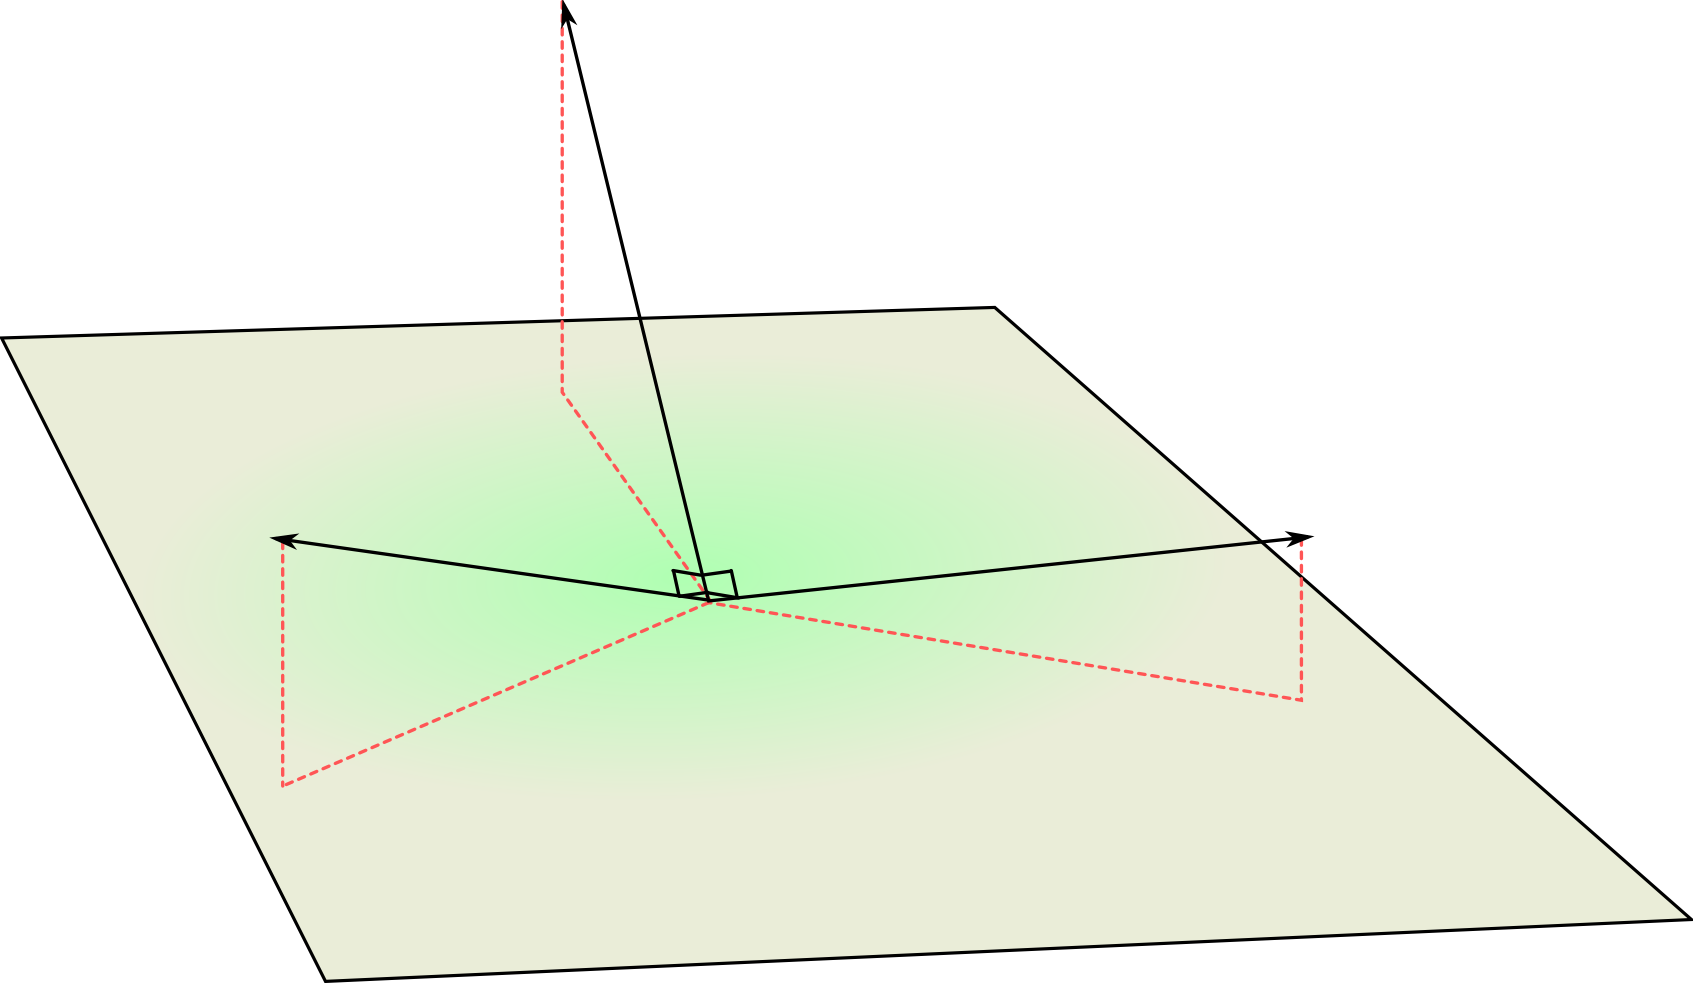
\includegraphics[width=0.6\textwidth]{fig/projection.png}
\label{fig:projection}
\caption{An informal demonstration of how the 3-D problem may be projected onto a 2-D domain.}
\end{figure}


\section{Coordinate Transformation}
\label{sec:analytical-np:transformation}

\begin{figure}[h]
\centering
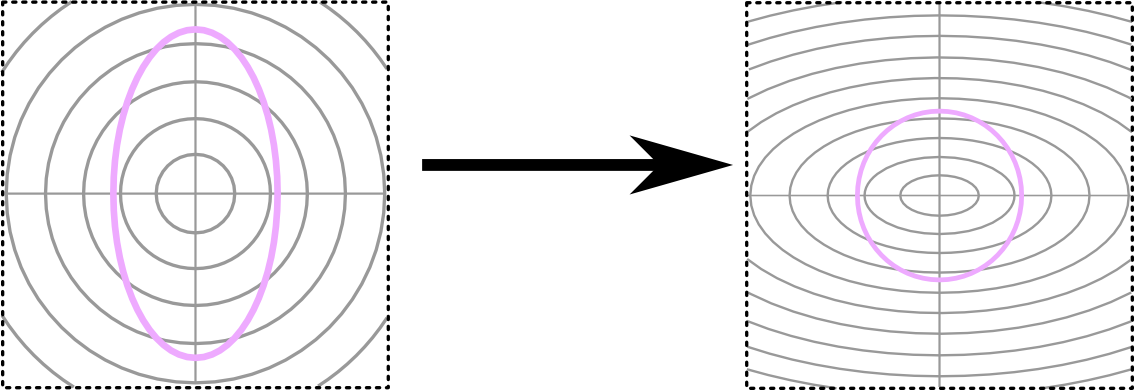
\includegraphics[width=0.8\textwidth]{fig/coordinate_transformation.png}
\label{fig:coord_trans}
\caption{A 2-dimensional linear coordinate transformation.}
\end{figure}

In order to apply the isotropic solution to this anisotropic case, we would like
to apply a coordinate transformation such that we can transform the problem into
an isotropic case with respect to some \(x' = a_x x\) and \(y' = a_y y\), as in
figure \ref{fig:coord_trans}.
Without loss of generality, suppose \(a_x = 1\).

\begin{align}
\frac{dx'}{dx} &= 1\\
\frac{dy'}{dy} &= a_y\\
\frac{\partial f}{\partial x} &= \frac{\partial f}{\partial x'}\frac{dx'}{dx} = \frac{\partial f}{\partial x'}\\
\frac{\partial f}{\partial y} &= \frac{\partial f}{\partial y'}\frac{dy'}{dy} = a_y\frac{\partial f}{\partial y'}\\
\nabla T &= \frac{\partial T}{\partial x'} \e_{x'} + a_y\frac{\partial T}{\partial y'} \e_{y'} \\
[K]\nabla T &= k_x\frac{\partial T}{\partial x'} \e_{x'} + k_ya_y\frac{\partial T}{\partial y'} \e_{y'}\\
\nabla \cdot \left([K]\nabla T\right) &= k_x\frac{\partial^2 T}{\partial {x'}^2} + k_ya_y^2\frac{\partial^2 T}{\partial {y'}^2}\\
\end{align}

Suppose we set the right side equal to the equivalent isotropic expression:
\begin{equation*}
k\left(\frac{\partial^2 T}{\partial {x'}^2} + \frac{\partial^2 T}{\partial {y'}^2} \right) = k_x\frac{\partial^2 T}{\partial {x'}^2} + k_ya_y^2\frac{\partial^2 T}{\partial {y'}^2}
\end{equation*}

As a result,

\begin{align*}
k &= k_x\\ a_y &= \sqrt{\frac{k_x}{k_y}}\\
\end{align*}

Therefore, the following coordinate transformation will allow us to apply the
isotropic solutions to an isotropic case with \(k = k_x\):

\begin{equation}
    \label{coord_trans}
    \begin{pmatrix}x' \\ y'\end{pmatrix} =
    \begin{bmatrix}1 & 0\\ 0 & \sqrt{\frac{k_x}{k_y}} \end{bmatrix}\begin{pmatrix}x \\ y\end{pmatrix}
\end{equation}

\section{From Temperature Distribution to Measurement}
\label{sec:analytical-np:isotropic}

Using equation \ref{coord_trans}, we may apply the isotropic solution:

\begin{equation}
    -k_x \nabla^2 T = \rho C\frac{\partial T}{\partial t}
\end{equation}

and get the following result (for sufficiently large \(t/r'\)):

\begin{equation}
T(r',t) = \frac{q}{4\pi k_x}\ln\left(\frac{4k_xt}{r'^2}\right) - \frac{\gamma q}{4\pi k_x}
\end{equation}

When measuring for the anisotropic case, I argue that we are effectively
measuring the temperature at some \(r = r_{\textrm{0}}\)---either on the surface
of the needle, or some small distance away from the needle.

Applying this technique to the anisotropic case, we find that we must also
transform \(r_{xy} = \cos(\theta) \hat{e}_x + \sin(\theta) \hat{e}_y \)
into \(r_{x'y'}\):

\begin{align*}
    \begin{pmatrix}r_{x'} \\ r_{y'}\end{pmatrix} &=
    \begin{bmatrix}1 & 0\\ 0 & \sqrt{\frac{k_x}{k_y}} \end{bmatrix}\begin{pmatrix}r_0\cos(\theta) \\ r_0\sin(\theta)\end{pmatrix}\\
    &= r_0\left(\cos(\theta) \e_x + \sqrt{\frac1{k_y}} \e_y \right)\\
\end{align*}
\begin{equation}
    \norm{r}^2 = r_0^2 \left(\cos^2(\theta) + \frac{k_x}{k_y}\sin^2(\theta) \right)\\
\end{equation}

This means that the temperature around the needle should now vary as a function
of \(\theta\), unlike in the isotropic case. Now, since the needle only measures
a single value, it seems logical to suggest that the measured quantity is an
average temperature---say, the average surface temperature of the probe.  This
may be expressed like so:

\begin{equation}
T_{\textrm{avg}}(t) = \frac{ \int_0^{2\pi} T(r,t) rd\theta }
                           { \int_0^{2\pi} rd\theta}
\end{equation}

I ended up simplifying it such that, where

\begin{equation}
\mathcal{E}(f(\phi, \alpha), \alpha) = \int_0^{2\pi} f\sqrt{\cos^2(\phi) + \alpha\sin^2(\phi)} d\phi
\end{equation}

we have

\begin{equation}
\frac{4\pi k_x}{q} \frac{\mathcal{E}(\ln(t), \frac{k_y}{k_x})}{\mathcal{E}(1, \frac{k_y}{k_x})}
\end{equation}

\section{Finding Measured Conductivity as a Function of Needle Orientation}
